\documentclass[conference]{IEEEtran}
\IEEEoverridecommandlockouts

\usepackage{cite}
\usepackage{amsmath,amssymb,amsfonts}
\usepackage{algorithmic}
\usepackage{graphicx}
\usepackage{textcomp}
\usepackage{xcolor}
\def\BibTeX{{\rm B\kern-.05em{\sc i\kern-.025em b}\kern-.08em
    T\kern-.1667em\lower.7ex\hbox{E}\kern-.125emX}}
\begin{document}

\title{
Using Reinforcement Learning to Learn Novel Strategies
for Collective Decision Making \\
\thanks{
This research was sponsored by the U.S. Army Research Laboratory
and the U.K. Ministry of Defence
under Agreement Number W911NF-16-3-0001.
The views and conclusions contained in this document are those of the authors
and should not be interpreted as representing the official policies,
either expressed or implied, of the U.S. Army Research Laboratory,
the U.S. Government, the U.K.  Ministry of Defence or the U.K. Government.
The U.S. and U.K. Governments are authorized to reproduce and distribute
reprints for Government purposes notwithstanding any copyright notation hereon.
}
}

\author{
\IEEEauthorblockN{Hugo McNally, Sebastian Stein}
\IEEEauthorblockA{\textit{Electronics and Computer Science} \\
\textit{University of Southampton}\\
Southampton, UK\\
\{hm6g17, s.stein\}@soton.ac.uk}
\and
\IEEEauthorblockN{Malgorzata Turalska}
\IEEEauthorblockA{\textit{Network Science Division} \\
\textit{CCDC Army Research Laboratory}\\
Adelphi, MD, USA \\
mg.turalska@gmail.com}
\and
\IEEEauthorblockN{Rosie Lickorish, Geeth De Mel}
\IEEEauthorblockA{\textit{IBM Research Europe} \\
\textit{IBM}\\
Hursley, UK \\
\{rosie.lickorish, geeth.demel\}@uk.ibm.com}
}

\maketitle

\begin{abstract}
In military settings, collaborative decision making
is often used to solve large and complex problems under time pressure.
Here, workers can adopt
particularly promising solutions found by colleagues (imitation)
or independently explore new solutions (innovation).
However, there exists a trade-off between imitation and individual innovation
which has a consequential impact on the quality of the final solution found.
Therefore, the design of effective collaboration strategies
is an important problem when trying to find good solutions
to large and complex problems.
This paper formulates this strategy design as a reinforcement learning problem
and presents preliminary results
showing that, over short time periods, reinforcement learning outperforms
most handcrafted heuristics that are typically used in these settings.
\end{abstract}
\begin{IEEEkeywords}
collective decision making, NK-landscapes, collective intelligence,
problem solving, reinforcement learning
\end{IEEEkeywords}

\section{Introduction}\label{intro}
Collaborative decision making is utilised by most organisations,
including the military,
to find good solutions to large problems.
This is achieved due
to the large number of agents working on the problem simultaneously
and their ability to either
imitate promising solutions of their colleagues or neighbours,
or to innovate and discover better solutions independently.

The choices of agents to imitate as opposed to innovate,
can have a substantial impact on the time taken
for a good solution to be reached
and on the quality of the final solution found.
Specifically there is a trade off between imitation and innovation,
with more imitation offering good solutions faster
but more innovation resulting in the better solution in the long run.
In addition to this,
the way in which an agent selects a neighbour to copy
also has a notable impact
\cite{monotonic, sociallearning}.

This existing body of research
has explored and evaluated strategies developed using heuristic methods.
Reinforcement learning has the potential to produce novel strategies.
Not only this, but reinforcement learning could be tasked with
learning strategies tailored for different problem complexities,
organisational structures and for given time budgets.
The differences in these strategies could offer invaluable insights
into how organisations adapt to different situations.

This paper preposes a way in which the collective learning scenarios
can be reframed as Finite Markov Decision Processes
and the preliminary results of a simple Q Learning approach,
before suggesting further research
which could be carried out in this area.


\section{Model}

An organisations can be modelled as a graph $G(w, e)$
which is searching for the optimal solution to a given problem,
where $w$ are the workers and $e$ are the edges between them.
Here, an edge signifies a collaborative relationship between two workers
(colleagues).

The problem is modelled as a NK landscape,
so has an integer solution space with the range $(0, N]$
and with a complexity increasing with $K$.
The problems are generated using the method from \cite{monotonic}.
The score allocated to each solution is passed through a monotonic function,
which skews scores lower,
to reflect that the majority of solutions
to real world problems are poor.

In this problem space,
individual innovation can be simulated
by a worker randomly flipping a bit of its current solution.
A step is only taken if the result of the bit flip is better
than the solution previously held by the agent.

The organisation solves the problem over discrete time steps
and the organisation's goal is to achieve
the best average performance among its workers
by the deadline.
Here, the deadline is the maximum number of time steps before an `episode' ends.


\section{Markov Decision Process}\label{mdp}

Reframing collective decision making as a Markov Decision Process
simply involves devising a way to express a worker's state
and provide actions which a worker is able to perform.

For the preliminary investigation,
three strategies are available to workers as actions:
\emph{best member imitation else step},
\emph{conformity imitation else step} and
\emph{step else best member imitation}.
Following the first, a worker would imitate the solution
of its colleague with the highest score.
However, if this colleague's score is not higher
than the worker's current score,
the worker will innovate taking a step.
The second is a similar process only the worker will attempt
to copy a neighbour
whose score is the same as one or more of the other neighbours.
Following the third strategy,
a worker would attempt to find a better solution by taking a random step,
before attempting to imitate its best neighbour.

Because the objective is to find a generalisable strategy
for problems of a given complexity,
the agent will learn over many different problems.
Therefore, the information attributed to an agent's position
on the landscape changes and so is not valuable.
The time step the worker is in, by contrast, lends itself well to being a state.
The worker's current score, its best performing colleague's score,
the mean of all colleagues' scores
and the variance in all its colleagues' scores
can all be added as additional dimensions to the state space.
All of these will provide likely valuable situational awareness to the agent.

This paper makes a distinction between a worker,
the organisation's components that can carry out an action,
and the agent,
the learning algorithm and resulting strategy model shared by all workers.


\section{Preliminary Results}\label{results}

For the preliminary experiments,
the Q learning algorithm \cite{qlearning} was used.
Initially the state space used was the current score
and the time step of the worker.
The worker scores were quantised into 50 levels.
However, this state space resulted in agents being incredibly slow to train,
which was likely due to quantisation.
With few solutions resulting in high scores due to the monotonic function,
high scores are rare.
A consequence of this is high score states being updated rarely,
reducing the agent's ability to learn the best actions to take at higher scores.
Because of this, the second set of experiments run used time step
as the only dimension of the state space.

\begin{figure}[htbp]
    \centering
    \centerline{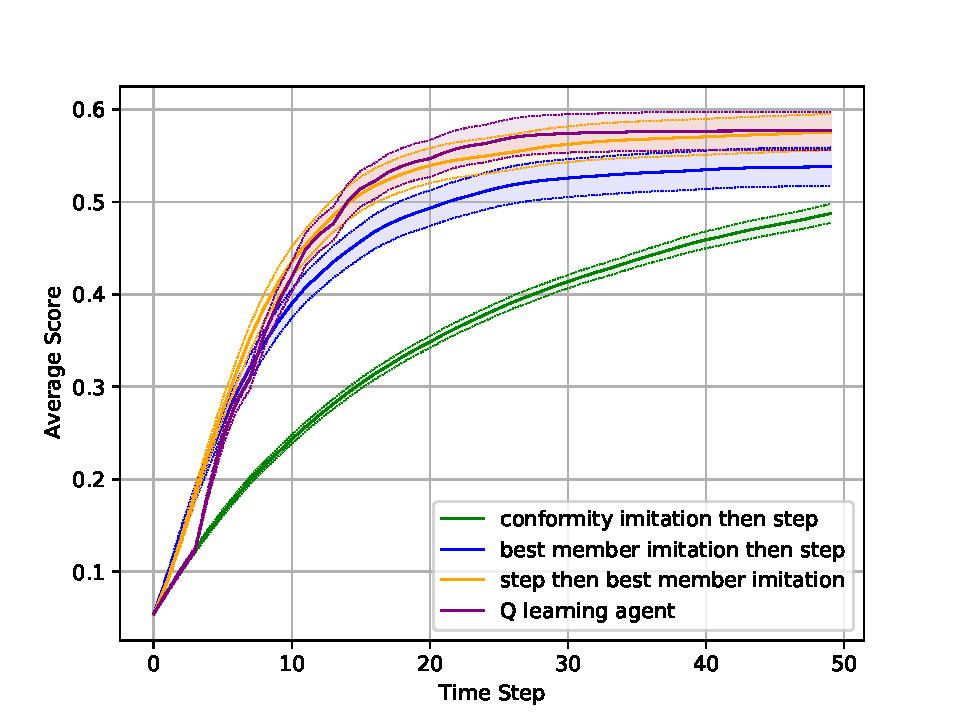
\includegraphics[scale=0.58]{figures/version4.pdf}}
    \caption{
        The average over 500 episodes of the agents' average score
        at each time step, with the 95\% confidence intervals
        plotted as dotted lines.
        Each episode a had a unique NK Landscape with N = 12 and K = 4
        and a regular graph with 60 workers each with 4 colleagues.
    }
    \label{avscore}
\end{figure}

The Q learning agent shown in Figure \ref{avscore}
used a epsilon greedy exploration with a epsilon decay from $1$ of $10^{-8}$,
had a learning rate of $0.6$ and a discount factor of $0.1$.
The agent was trained in for regular graph with 60 workers
each with 4 colleagues, on random NK Landscapes with N = 12 and K = 4,
and with a deadline of 50 time steps.

After training for 90100 episodes, around 7 hours of training,
it can be seen to perform marginally better
than the best of the individual strategies after time step 14.

Although the agent does not show a considerable performance improvement
over the individual strategies,
it exbibits a very promising trait.
It adherence to \emph{conformity imitation then step}
in the first few time steps,
a strategy known to keep the number of unique solutions
high \cite{sociallearning}.
This suggests the agent has learnt to avoid
clustering workers into similar solutions early in the episode,
and seems to have enabled the agent to subsequently outperform
the individual strategies at time step 15.

The reward was issued at each step as the improvement in the worker's score.
The agent could be better incentivised to get the maximum score at the deadline,
by only issuing the final worker score as a reward.


\section{Future Work}
Reinforcement learning shows promise
in its ability to identity good strategies for collective decision making.
Given more time experimenting with different
states spaces, actions spaces and learning techniques,
it is likely that reinforcement learning could offer valuable insights
into the best strategies to approach different problems with.

Another potentially promising approach is to provide agents
with the components of a strategy (e.g. \emph{step}) as actions
and then, once training is complete, the agent can attempt the $n$ actions
with the highest perceived value in order of value.
This would allow agents more flexibility in strategy design
and has the potential to produce more novel strategies.

Environment noise will be a major factor in
the current Q Learning agent's sluggish learning.
This noise is due to the generation of a random NK landscapes for each episode,
each of which can favour very different strategies.
G Learning \cite{glearning}
could offer a solution to this problem.
It mitigates the tendency of Q Learning to form a bias.
Not only this, but G Learning allows a prior to be used,
which could be handcrafted heuristics from research.


\bibliography{refs}{}
\bibliographystyle{unsrt}


\end{document}
